\section{Accounts and Enrolments}
\subsection{Overview}
The ability to create and manage accounts and enrollments of students, teachers and administrators is a key feature of any LMS. Without being able to create and manage individual accounts for each type of user, the system will be impractical for use in educational environments, and without being able to enroll into courses and topics, many other features of our Meta LMS will not be useful.

There are 4 main pages relating to accounts and enrollment:
\begin{itemize}
  \item Sign in and sign up;
  \item Viewing and editing account details;
  \item administrators enrolling students and creating course invite codes; and,
  \item Students self-enrolling.
\end{itemize}

\textbf{Sign in and sign up}

The sign in and sign up screens need to allow users to enter the necessary details to either sign in or sign up, while also being as accessible as possible. Many designs already exist for these components so it is a matter of utilizing the features of existing designs that support accessibility the most. These features include high contrast colors, large readable text, a clear page flow and sufficient text instructions.

\begin{figure}[h!]
  \centering
  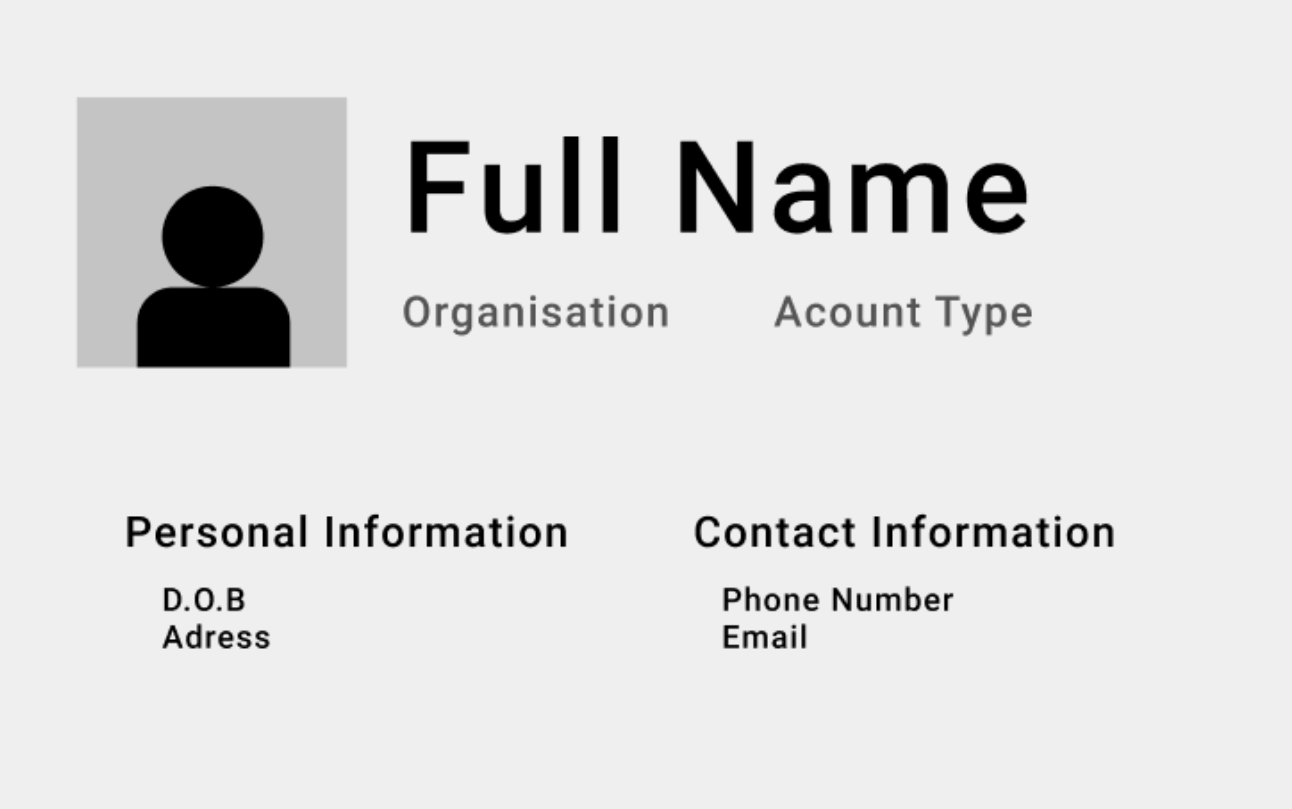
\includegraphics[scale=0.2]{images/accounts-profile}
  \caption{A user's view of their account.}
\end{figure}

\textbf{Viewing and Editing Account Details}

User's need to be able to easily view their account information, and that of other users. Accessibility is a key concern for this page, so a clear page flow and easy to read text are most important, as well as a sleek and visually appealing user interface to ensure that information can be comprehended from the page as easily as possible.

\begin{figure}[h!]
  \centering
  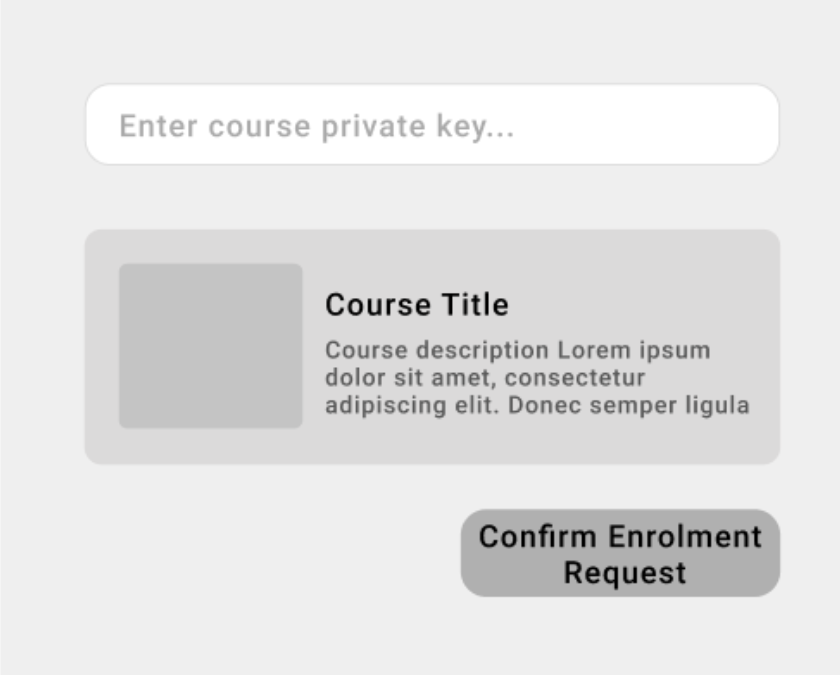
\includegraphics[scale=0.2]{images/accounts-code}
  \caption{A student user's screen to enrol in a course via invite code.}
\end{figure}

\textbf{Administrators Enrolling Students}

administrators need to be able to individually add student's to a course, and generate an invite code that students can use to enroll in a course. 

\begin{figure}[h!]
  \centering
  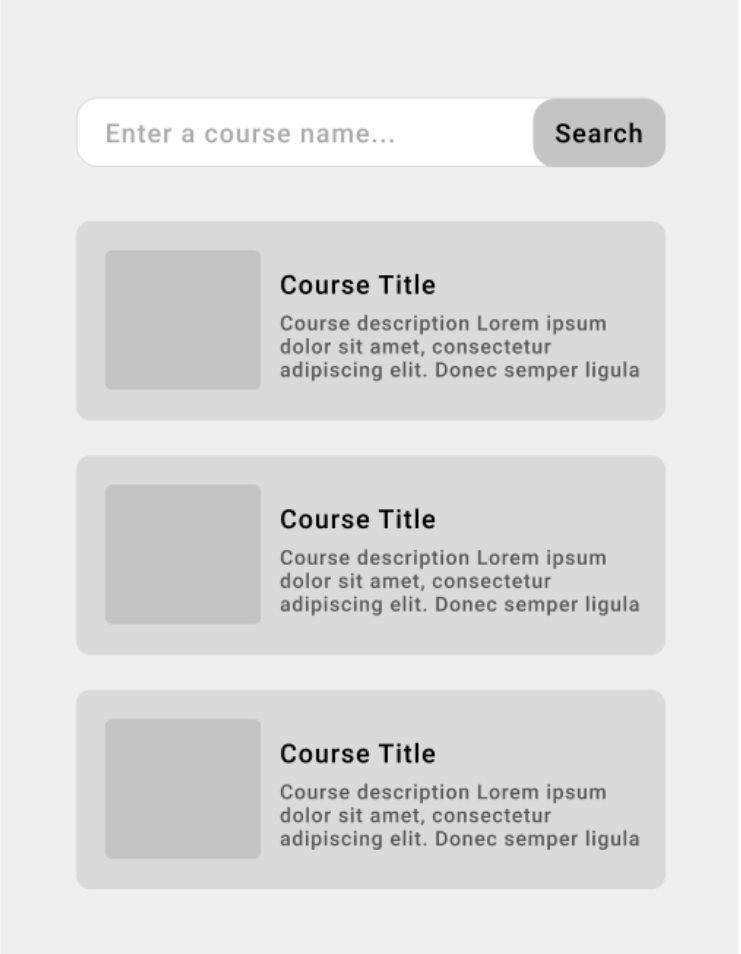
\includegraphics[scale=0.2]{images/accounts-search}
  \caption{A student user's view to search for courses and topics.}
\end{figure}

\textbf{Student's Self Enrolling}

A student user needs to be able to either enter a course invite code generated by an administrator, or search for a course or topic via its name or course code, to enroll themselves into a course. It is important that when searching for courses and topics, as much information is as clearly displayed as possible.

The accounts system is also in charge of governing the data of the different users. Thus it is important to plan the design of the database schema for a user account. Below is an initial design of what the database table headings for a user may look like:

\begin{center}
    \begin{tabular}{|c|c|c|c|c|c|c|c|} 
        \hline
        id & type & name & email & password & phone & address & topics \\ [0.5ex] 
        \hline
    \end{tabular}
\end{center}

The ID field has dual purposes, it both stores a users student ID, and is also a unique identifier for every student. The type field stores the account type of a user, such as student or administrator. We also need to be able to store a users personal information, such as their name, phone number and address so there are fields for that. The user needs to be able to log in so an email and password will also be stored. Finally a list of all of the topics a user has completed must also be stored so that their progress can be reflected in any courses they are enrolled in.\\


\subsection{Additional Features and Refinements}

No additional features were added throughout developments to the accounts and enrollment feature, however many of the design decisions were altered and refined as development and testing caused new issues to be identified. For example the initial database schema above changed during development. It became apparent that this schema would not meet the needs of the LMS in terms of storing user data. This new schema was what was decided on:
\begin{center}
    \begin{tabular}{|c|c|c|c|c|c|c|c|c|} 
        \hline
        id & type & name & email & password & studentID & staff & img\_url & last\_accessed\_topic \\ [0.5ex] 
        \hline
    \end{tabular}
\end{center}
The phone number and address fields were removed, as it became apparent that it was not necessary to store this information for the functionality of the LMS. The topic groups column was also removed as the notion of enrollment was moved to its own table to enhance functionality. The user's id was separated from their student ID, to prevent issues with storing data, and an img\_url field was added to store the user's profile picture. The last accessed\_topic\_field was also added so that this information could be stored to be displayed on a users dashboard to create a more personal user experience. 

\subsection{Requirements}
The initial requirements for the accounts and enrolment system are listed below. Each requirement has a priority that was measured by surveying the other thesis members. Higher priority items will be completed first, with medium and then low priority requirements to be implemented later in the project in their respective order.

The initial list of requirements were broken up into accounts and enrollments, and were as follows:

\textbf{Accounts}

    \begin{enumerate}
    \item Users can register and login \textcolor{Red}{High}
    \item Users can view and update their details \textcolor{Red}{High}
    \item administrators can manage users, roles and permissions \textcolor{Red}{Medium}
    \item administrators can create accounts on behalf of students \textcolor{Orange}{Medium}
    \item administrators can view other users account details \textcolor{Orange}{Medium}
    \end{enumerate}

\textbf{Enrollments}

    \begin{enumerate}
    \item administrators can open and close enrolments for courses \textcolor{Red}{High}
    \item administrators can enrol and un-enroll students on their behalf \textcolor{Red}{High}
    \item administrators can generate course invite codes \textcolor{Red}{High}
    \item administrators can set courses to be open enrolment or invite/code only \textcolor{Orange}{Medium}
    \item Students can enrol themselves in courses with a code \textcolor{Red}{High}
    \item Students can enrol themselves in an open course or topic \textcolor{Red}{High}
    \item Students can search for open courses \textcolor{Blue}{Low}
    \end{enumerate}

However, as the project progressed, it became clear that it did not make sense to keep these requirements divided like this, and that some of the priorities were incorrect compared to the importance of the requirement to the LMS. The requirements were instead adjusted in priority and refined to have acceptance criteria as follows:

\textbf{Login and Sign Up}

Users can register and login \textcolor{Red}{High}
\begin{center}
    \begin{tabular}{|ll|}
    \hline
        \multicolumn{1}{|l|}{\textbf{AS A}}      & User \\ \hline
        \multicolumn{1}{|l|}{\textbf{I WANT TO}} & Create a new account and log in to my existing account \\ \hline
        \multicolumn{1}{|l|}{\textbf{SO THAT}}   & I can use the LMS \\ \hline
        \multicolumn{2}{|l|}{\textbf{Acceptance Criteria:}} \\ \hline
        \multicolumn{2}{|l|}{\begin{tabular}[c]{@{}l@{}}- The user can successfully sign up to the LMS\\ - The user can use an account previously made to log in\end{tabular}} \\ \hline
    \end{tabular}
\end{center}

Staff can create accounts on behalf of students \textcolor{Blue}{Low}
\begin{center}
\begin{tabular}{|ll|}
\hline
\multicolumn{1}{|l|}{\textbf{AS A}}                                    & Staff Member                                                                             \\ \hline
\multicolumn{1}{|l|}{\textbf{I WANT TO}}                               & Create accounts on behalf of students                                                    \\ \hline
\multicolumn{1}{|l|}{\textbf{SO THAT}}                                 & I can streamline the formation of a course for new students                              \\ \hline
\multicolumn{2}{|l|}{\textbf{Acceptance Criteria:}}                                                                                                               \\ \hline
\multicolumn{2}{|l|}{\begin{tabular}[c]{@{}l@{}}- The staff can create a batch of student accounts\\ - Students can use these accounts to log in\end{tabular}} \\ \hline
\end{tabular}
\end{center}

\textbf{Account Management}

Users can view and update their details \textcolor{Orange}{Medium}
\begin{center}
\begin{tabular}{|ll|}
\hline
\multicolumn{1}{|l|}{\textbf{AS A}}                                                    & User                                                                                    \\ \hline
\multicolumn{1}{|l|}{\textbf{I WANT TO}}                                               & View and update my details                                                              \\ \hline
\multicolumn{1}{|l|}{\textbf{SO THAT}}                                                 & I can ensure my information is up to date                                               \\ \hline
\multicolumn{2}{|l|}{\textbf{Acceptance Criteria:}}                                                                                                                              \\ \hline
\multicolumn{2}{|l|}{\begin{tabular}[c]{@{}l@{}}- Users can access a page that shows their account information\\ - Users can edit their information from this page\end{tabular}} \\ \hline
\end{tabular}
\end{center}

Staff can manage other users \textcolor{Blue}{Low}
\begin{center}
\begin{tabular}{|ll|}
\hline
\multicolumn{1}{|l|}{\textbf{AS A}}                                           & Staff member                                                                                        \\ \hline
\multicolumn{1}{|l|}{\textbf{I WANT TO}}                                      & Manage other users                                                                                  \\ \hline
\multicolumn{1}{|l|}{\textbf{SO THAT}}                                        & I can ensure student's accounts contain the correct information                                     \\ \hline
\multicolumn{2}{|l|}{\textbf{Acceptance Criteria:}}                                                                                                                                 \\ \hline
\multicolumn{2}{|l|}{\begin{tabular}[c]{@{}l@{}}- Staff can access a page that shows a students account information\\ - They can edit this information from this page\end{tabular}} \\ \hline
\end{tabular}
\end{center}

\textbf{Enrollment Dashboard - Staff}

Staff can enrol and un-enroll students on their behalf \textcolor{Red}{High}
\begin{center}
\begin{tabular}{|ll|}
\hline
\multicolumn{1}{|l|}{\textbf{AS A}}                                                                   & Staff member                                                                                                 \\ \hline
\multicolumn{1}{|l|}{\textbf{I WANT TO}}                                                              & Enrol and un-enroll students from a course                                                               \\ \hline
\multicolumn{1}{|l|}{\textbf{SO THAT}}                                                                & I can effectively manage a course's enrollments                                                              \\ \hline
\multicolumn{2}{|l|}{\textbf{Acceptance Criteria:}}                                                                                                                                                                  \\ \hline
\multicolumn{2}{|l|}{\begin{tabular}[c]{@{}l@{}}- Staff can access a page that shows all students enrolled in a course\\ - They can enroll new students or un-enroll existing students from the course\end{tabular}} \\ \hline
\end{tabular}
\end{center}

Staff can generate course invite codes \textcolor{Red}{High}
\begin{center}
\begin{tabular}{|ll|}
\hline
\multicolumn{1}{|l|}{\textbf{AS A}}                                                                                                                       & Staff member                                                                                                                                                     \\ \hline
\multicolumn{1}{|l|}{\textbf{I WANT TO}}                                                                                                                  & Generate course invite codes                                                                                                                                     \\ \hline
\multicolumn{1}{|l|}{\textbf{SO THAT}}                                                                                                                    & I can effectively manage a course's enrollments                                                                                                                  \\ \hline
\multicolumn{2}{|l|}{\textbf{Acceptance Criteria:}}                                                                                                                                                                                                                                                                          \\ \hline
\multicolumn{2}{|l|}{\begin{tabular}[c]{@{}l@{}}- Staff can access a page that allows them to generate and manage course invite codes\\ - They can add restrictions to code like number of uses and time valid\\ - They can manage existing codes\\ - When a student uses the code they can enroll in a course\end{tabular}} \\ \hline
\end{tabular}
\end{center}

Staff can set courses to be open enrolment or invite/code only \textcolor{Red}{High}
\begin{center}
\begin{tabular}{|ll|}
\hline
\multicolumn{1}{|l|}{\textbf{AS A}}                                                              & Staff member                                                                                                 \\ \hline
\multicolumn{1}{|l|}{\textbf{I WANT TO}}                                                         & Set courses to be open enrolment or invite/code only                                                         \\ \hline
\multicolumn{1}{|l|}{\textbf{SO THAT}}                                                           & I can effectively manage a course's enrollments                                                              \\ \hline
\multicolumn{2}{|l|}{\textbf{Acceptance Criteria:}}                                                                                                                                                             \\ \hline
\multicolumn{2}{|l|}{\begin{tabular}[c]{@{}l@{}}- Staff can access a page that allows them to manage whether a course is publically search-able\\ - They can control whether a course is public\end{tabular}} \\ \hline
\end{tabular}
\end{center}


\textbf{Enrollment Dashboard - Student}

Students can enrol themselves in courses with a code \textcolor{Red}{High}
\begin{center}
\begin{tabular}{|ll|}
\hline
\multicolumn{1}{|l|}{\textbf{AS A}}                                                                                       & Student                                                                                                              \\ \hline
\multicolumn{1}{|l|}{\textbf{I WANT TO}}                                                                                  & Enrol myself in courses with a code                                                                                  \\ \hline
\multicolumn{1}{|l|}{\textbf{SO THAT}}                                                                                    & I can enroll in a new course                                                                                         \\ \hline
\multicolumn{2}{|l|}{\textbf{Acceptance Criteria:}}                                                                                                                                                                                              \\ \hline
\multicolumn{2}{|l|}{\begin{tabular}[c]{@{}l@{}}- Students have access to an enrollment page where they can enroll in a course with an invite code\\ - After submitting the code, they are enrolled in the corresponding course\end{tabular}} \\ \hline
\end{tabular}
\end{center}

Students can search for open courses \textcolor{Red}{High}
\begin{center}
\begin{tabular}{|ll|}
\hline
\multicolumn{1}{|l|}{\textbf{AS A}}                                                                                                          & Student                                                                                                                          \\ \hline
\multicolumn{1}{|l|}{\textbf{I WANT TO}}                                                                                                     & Search for open courses                                                                                                          \\ \hline
\multicolumn{1}{|l|}{\textbf{SO THAT}}                                                                                                       & I can enroll in a new course                                                                                                     \\ \hline
\multicolumn{2}{|l|}{\textbf{Acceptance Criteria:}}                                                                                                                                                                                                                             \\ \hline
\multicolumn{2}{|l|}{\begin{tabular}[c]{@{}l@{}}- Students have access to an enrollment page where they can search for courses\\ - After searching, a list of courses will be shown to the student\\ - Students can interact with this list to enroll in a course\end{tabular}} \\ \hline
\end{tabular}
\end{center}

The priority of the enrollment features for both staff and students were all increased to high priority due to the discovery of their importance to the entire LMS during development and internal testing. Without these features, the LMS becomes non-functional and thus they needed to be included. The admin management of student accounts was lowered in priority, as it became clear that these features were not essential to the functionality of the LMS, and if they did not manage to be completed it would not affect the functionality of the overall LMS too greatly.

In addition to assessing how well the accounts and enrolments features meet the requirements specified above, it will also be evaluated on how well it meets the following criteria:
\begin{enumerate}
    \item Performance - Whether it is quick to create an account or sign-up, and the responsiveness of the enrolment features.
    \item Accessibility - Can a wide array of users easily navigate account management areas and enrolment forms.
\end{enumerate}
The software tool Google Lighthouse will be used to evaluate these metrics. Google lighthouse uses automated tests to asses the response time of the page, and then analyses the code executed to build the page to find what may be causing a page to take a long time to respond and render. It also uses this same analysis to determine whether best accessibility practices have been used such as using appropriate alt-tags and aria labels where possible, and ensuring that components have proper contrast.